\documentclass[aspectratio=169]{../latex_main/tntbeamer}  % you can pass all options of the beamer class, e.g., 'handout' or 'aspectratio=43'
\usepackage{dsfont}
\usepackage{bm}
\usepackage[english]{babel}
\usepackage[T1]{fontenc}
%\usepackage[utf8]{inputenc}
\usepackage{graphicx}
\graphicspath{ {./figures/} }
\usepackage{algorithm}
\usepackage[ruled,vlined,algo2e,linesnumbered]{algorithm2e}
\usepackage{hyperref}
\usepackage{booktabs}
\usepackage{mathtools}

\usepackage{amsmath,amssymb}

\DeclareMathOperator*{\argmax}{arg\,max}
\DeclareMathOperator*{\argmin}{arg\,min}

\usepackage{pgfplots}
\pgfplotsset{compat=1.16}
\usepackage{tikz}
\usetikzlibrary{trees} 
\usetikzlibrary{shapes.geometric}
\usetikzlibrary{positioning,shapes,shadows,arrows,calc,mindmap}
\usetikzlibrary{positioning,fadings,through}
\usetikzlibrary{decorations.pathreplacing}
\usetikzlibrary{intersections}
\pgfdeclarelayer{background}
\pgfdeclarelayer{foreground}
\pgfsetlayers{background,main,foreground}
\tikzstyle{activity}=[rectangle, draw=black, rounded corners, text centered, text width=8em]
\tikzstyle{data}=[rectangle, draw=black, text centered, text width=8em]
\tikzstyle{myarrow}=[->, thick, draw=black]

% Define the layers to draw the diagram
\pgfdeclarelayer{background}
\pgfdeclarelayer{foreground}
\pgfsetlayers{background,main,foreground}

% Requires XeLaTeX or LuaLaTeX
\usepackage{unicode-math}

\usepackage{fontspec}
%\setsansfont{Arial}
\setsansfont{RotisSansSerifStd}[ 
Path=../latex_main/fonts/,
Extension = .otf,
UprightFont = *-Regular,  % or *-Light
BoldFont = *-ExtraBold,  % or *-Bold
ItalicFont = *-Italic
]
\setmonofont{Cascadia Mono}[
Scale=0.8
]

% scale factor adapted; mathrm font added (Benjamin Spitschan @TNT, 2021-06-01)
%\setmathfont[Scale=1.05]{Libertinus Math}
%\setmathrm[Scale=1.05]{Libertinus Math}

% other available math fonts are (not exhaustive)
% Latin Modern Math
% XITS Math
% Libertinus Math
% Asana Math
% Fira Math
% TeX Gyre Pagella Math
% TeX Gyre Bonum Math
% TeX Gyre Schola Math
% TeX Gyre Termes Math

% Literature References
\newcommand{\lit}[2]{\href{#2}{\footnotesize\color{black!60}[#1]}}

%%% Beamer Customization
%----------------------------------------------------------------------
% (Don't) Show sections in frame header. Options: 'sections', 'sections light', empty
\setbeamertemplate{headline}{empty}

% Add header logo for normal frames
\setheaderimage{
	% 
\includegraphics[height=\logoheight]{figures/TNT_darkv4.pdf}
	
\includegraphics[height=\logoheight]{../latex_main/figures/luh_logo_rgb_0_80_155.pdf}
	% 
\includegraphics[height=\logoheight]{figures/logo_tntluh.pdf}
}

% Header logo for title page
\settitleheaderimage{
	% 
\includegraphics[height=\logoheight]{figures/TNT_darkv4.pdf}
	
\includegraphics[height=\logoheight]{../latex_main/figures/luh_logo_rgb_0_80_155.pdf}
	% 
\includegraphics[height=\logoheight]{figures/logo_tntluh.pdf}
}

% Title page: tntdefault 
\setbeamertemplate{title page}[tntdefault]  % or luhstyle
% Add optional title image here
%\addtitlepageimagedefault{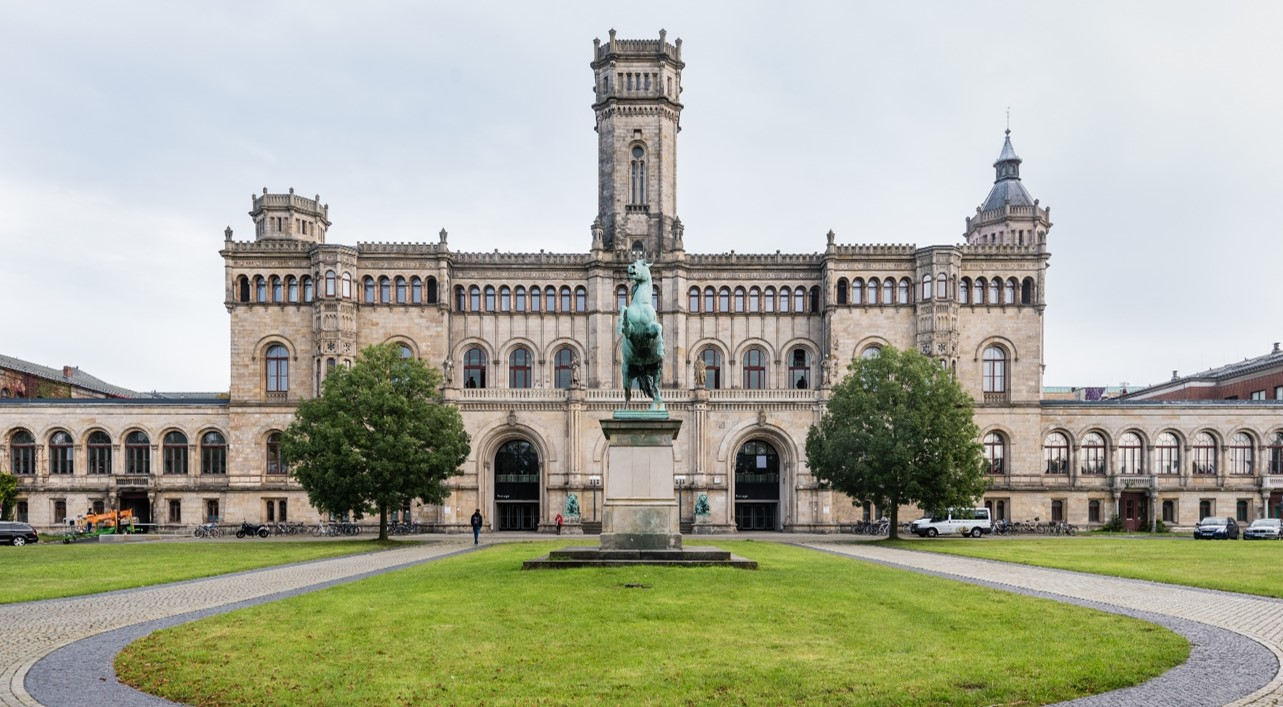
\includegraphics[width=0.65\textwidth]{figures/luh_default_presentation_title_image.jpg}}

% Title page: luhstyle
% \setbeamertemplate{title page}[luhstyle]
% % Add optional title image here
% \addtitlepageimage{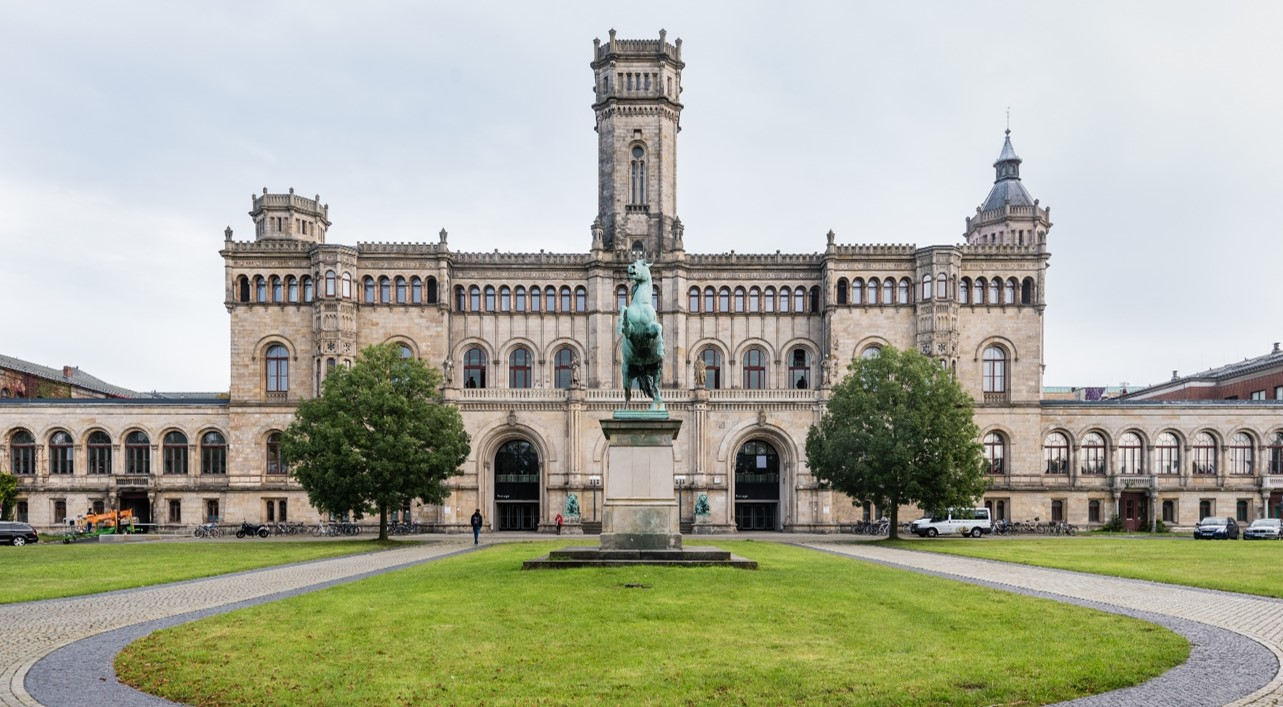
\includegraphics[width=0.75\textwidth]{figures/luh_default_presentation_title_image.jpg}}

\author[Lindauer \& Anand]{Marius Lindauer and Avishek Anand\\[1em]
	
\includegraphics[height=\logoheight]{../latex_main/figures/luh_logo_rgb_0_80_155.pdf}\qquad

\includegraphics[height=\logoheight]{../latex_main/figures/TNT_darkv4}\qquad

\includegraphics[height=\logoheight]{../latex_main/figures/L3S.jpg}	}
\date{Winter Term 2021
}


%%% Custom Packages
%----------------------------------------------------------------------
% Create dummy content
\usepackage{blindtext}

% Adds a frame with the current page layout. Just call \layout inside of a frame.
\usepackage{layout}


\title[Introduction]{iML: Local Explanations}
\subtitle{Pitfalls}

%\institute{}


\begin{document}
	
	\maketitle

	%-----------------------------------------------------------------------------------------------------------------------------
\begin{frame}{LIME Pitfalls \lit{Kopper and Molnar. 2019}{https://compstat-lmu.github.io/iml_methods_limitations/}}
  \begin{itemize}
  	\item LIME is one of the best known interpretable machine learning methods but several papers caution to be careful in their use. 
  \end{itemize}
	\textbf{Pitfall 1: Sampling}
	\begin{itemize}
	  \item The most common sampling strategies for $z \in Z$ do not take the correlation between features into account. 
      \item[$\leadsto$] unlikely data points which can then be used to learn local explanation models.
      \item Ideally, we need a local sampler that samples $z$ from $\mathcal{X}$. However, its derivation is particularly difficult for high dimensional or mixed feature spaces. 
      \item We could use the original training data to fit the surrogate model, but this only works well with enough data near $x$.
    \end{itemize}
\end{frame}

\begin{frame}{LIME Pitfalls \lit{Kopper and Molnar. 2019}{https://compstat-lmu.github.io/iml_methods_limitations/}}
\vspace{-2em}
	\textbf{Pitfall 2: Locality}
	\begin{itemize} 
     \item It is difficult to define locality (= how samples are weighted locally). %It has a huge influence on the local model, but there is no automatic procedure for choosing the neighborhood.
     \item The authors of LIME proposed an exponential kernel as proximity measure between $x$ and $z$
     	 \begin{center}
     		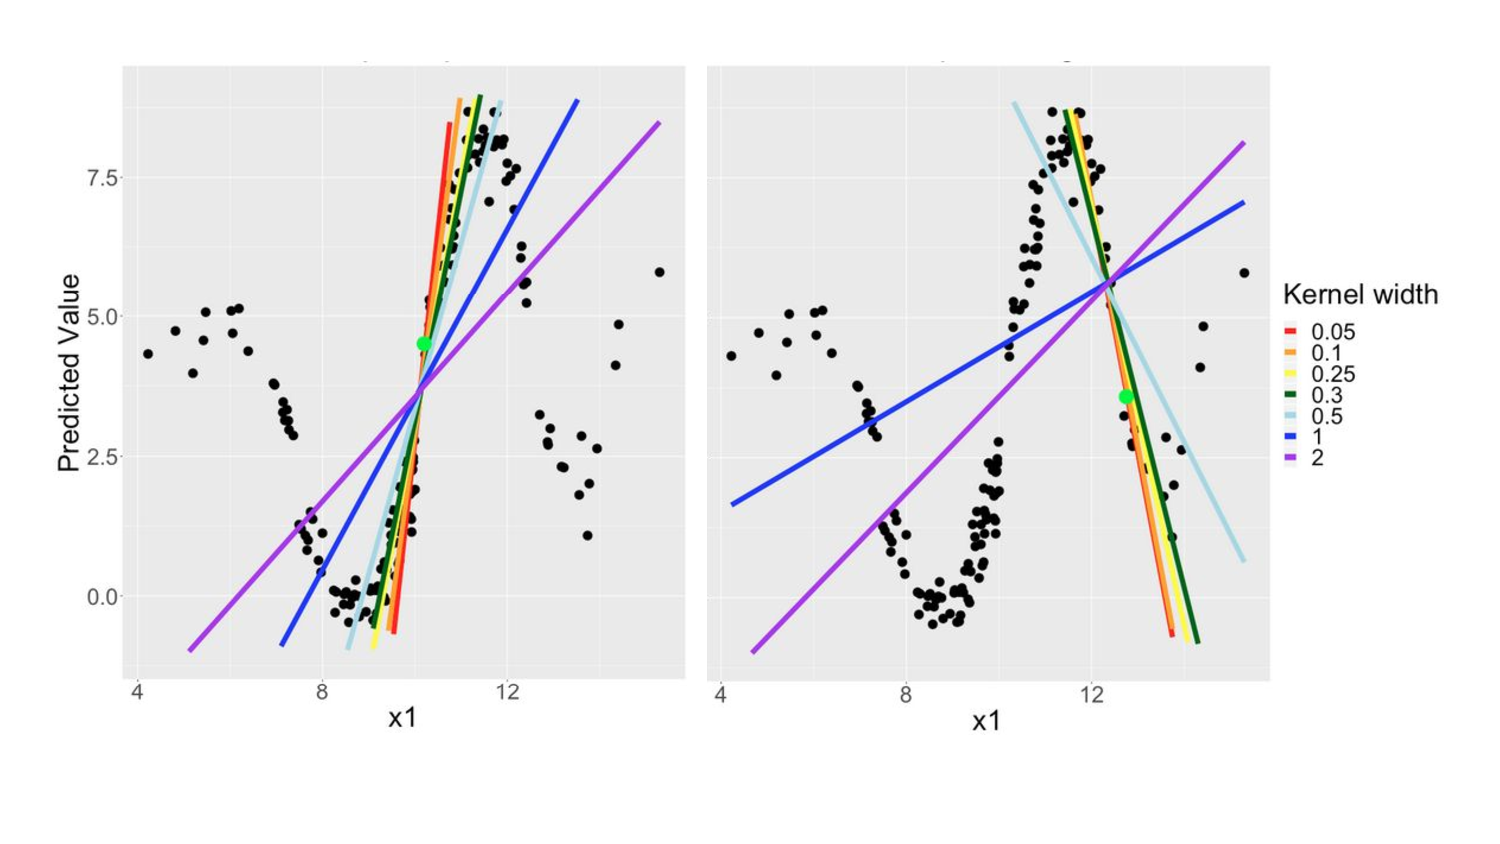
\includegraphics[width=0.4\textwidth]{figure/lime_locality}
     		%\scriptsize{\textbf{Figure:} Linear surrogate models for two different data points based on the same model with one target and one feature. Each line displays one linear surrogate model with a different kernel width. For the data point in the right figure, larger kernel sizes are more severe.}
     	\end{center}
     \item A larger kernel width means that instances that are farther away also influence the model such that we do not receive a local but a global surrogate model. 
     \item Prefer smaller kernel widths s.t. an instance must be very close to influence the local model.  
     \item If the kernel width is set too small, we only fit a local model based on a few observations which carries the risk to fit noise.   
	\item Multiple software package use another default standardized distance: the Gower proximity where no kernel width needs to be specified. However, experiments showed that since also data points far away receive a weight $ > 0$, their resulting explanations are rather global surrogates than local surrogates.   
\end{itemize}

\end{frame}

\begin{frame}{LIME Pitfalls \lit{Laugel et al. 2018}{http://webia.lip6.fr/~laugel/files/WHI_ICML_slides.pdf}}

\textbf{Pitfall 3: Local vs. global features}

\begin{columns}
	\begin{column}{0.78\textwidth}
\begin{itemize}
	\item There are features that influence the \textbf{global} shape of the black-box model and \textbf{local} features that impact predictions for a small area of $\mathcal{X}$. 
	\item For example in decision trees, splitting variables close to the root have a more global influence than the ones close to the leaves. 
	\item In most implementations, instances for the surrogate model are sampled from the whole input space which tends to hide the features with a local influence for the benefit of features with a global influence even when the kernel width was reduced. 
	\item Laugel et al. (2018) propose to sample new instances $z$ around the decision boundary closest from point $x$ for higher local accuracy.
\end{itemize}
\end{column}

\begin{column}{0.2\textwidth}

			\vspace{-0.2cm}
		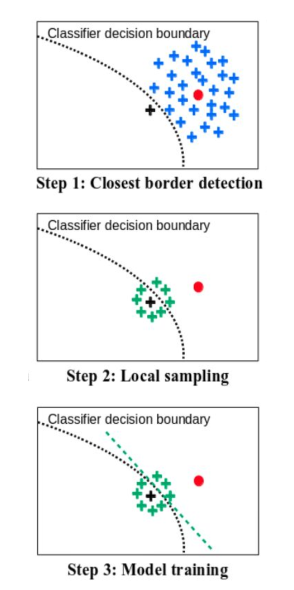
\includegraphics[width=1.\textwidth]{figure/lime_bordersample2}
		
 	\end{column}
\end{columns}

\end{frame}
% %-----------------------------------------------------------
% \begin{frame}[c]{LIME Pitfalls \lit{Laugel et al. 2018}{https://arxiv.org/pdf/1806.07498.pdf}}

% \begin{columns}
% 	\begin{column}{0.6\textwidth}
% 		\begin{itemize}
% 		\item Let us explain the prediction of the green dot. Background colors display predictions of a random forest, the gray line is the decision boundary.
% 		\item The decision boundary of LIME with default kernel width (green line) and reduced kernel width (blue line) do not match the direction of the steeper local boundary. 
% 		\item The method of Laugel et al. (2018) (red line) approximates the local border direction better. The red dot is the point closest to the border detected by this method. 
% 	\end{itemize}
% \end{column}
% \begin{column}{0.39\textwidth}
% \vspace{0.3cm}

% 	\begin{center}
% 	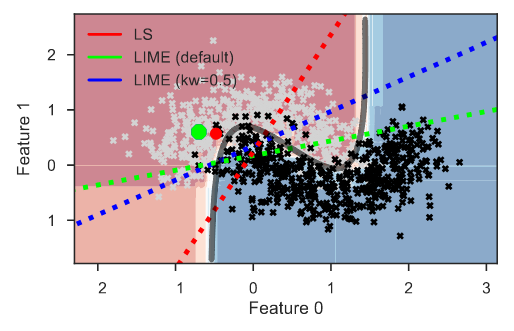
\includegraphics[width=1.0\textwidth]{figure/lime-globallocal2}
	
% 	\vspace{-0.3cm}
% 	{\tiny Half-moons dataset.}
	
% \end{center}

% 	\end{column}
% \end{columns}

% \end{frame}

\begin{frame}[c]{LIME Pitfalls \lit{Slack et al. 2020}{https://arxiv.org/abs/1911.02508}}
\textbf{Pitfall 4: Faithfulness}
\begin{itemize}
	\item There exists a trade-off between local fidelity vs. sparsity. 
	\item If the local fidelity of our interpretable model is low, we do not receive reliable explanations.
	\item On the other hand, high fidelity is only possible with a more complex model bearing the risk to substitute a black-box by complex model that is difficult to interpret.
\end{itemize}

\end{frame}
\begin{frame}{LIME Pitfalls \lit{Slack et al. 2020}{https://arxiv.org/abs/1911.02508}}
\vspace{-1em}
\textbf{Pitfall 5: Possibility to hide biases}
\begin{itemize}
	\item Data scientists could manipulate their model to hide biases. 
	\item Sampled instances for the surrogate model could be out of the input data distribution\\ if we do not account for feature dependencies. 
	\pause
	\item Build a classifier that detects whether a given data point is an out-of-distribution sample or not using the original training data and data sampled by LIME. 
	\item If a new data point has the same distribution as the training data, the prediction of the biased classifier is returned. If a new data point is out-of-distribution (usually samples for the surrogate models), the unbiased prediction is returned.
	\pause
	\item For the credit dataset, a biased model could be a model solely trained on the feature `gender`, while an unbiased model could be trained on features uncorrelated with `gender`.
	\item Since the surrogate model is trained on out-of-distribution samples, the predictions of these samples are derived from an unbiased predictor. 
	\item Consequently, the explanations do not detect any bias although the original predictor is biased. 
\end{itemize}
\end{frame}

\begin{frame}{LIME Pitfalls \lit{Alvarez-Melis and Jaakkola}{https://arxiv.org/abs/1806.08049}}
\vspace{-1em}
\textbf{Pitfall 6: Robustness}
\begin{itemize}
	\item Instability of the explanations. 
	\item Explanations of two very close points could vary greatly. 
	\item But also if $\hat{f}$ and $x$ are fixed, and only new sampled data points $z$ are used, the resulting explanations could differ. $\leadsto$ \alert{Rashomon Effect}. 
\end{itemize}
\vspace{-0.7cm}
\begin{columns}
	\begin{column}{0.48\textwidth}
		\begin{center}
		
		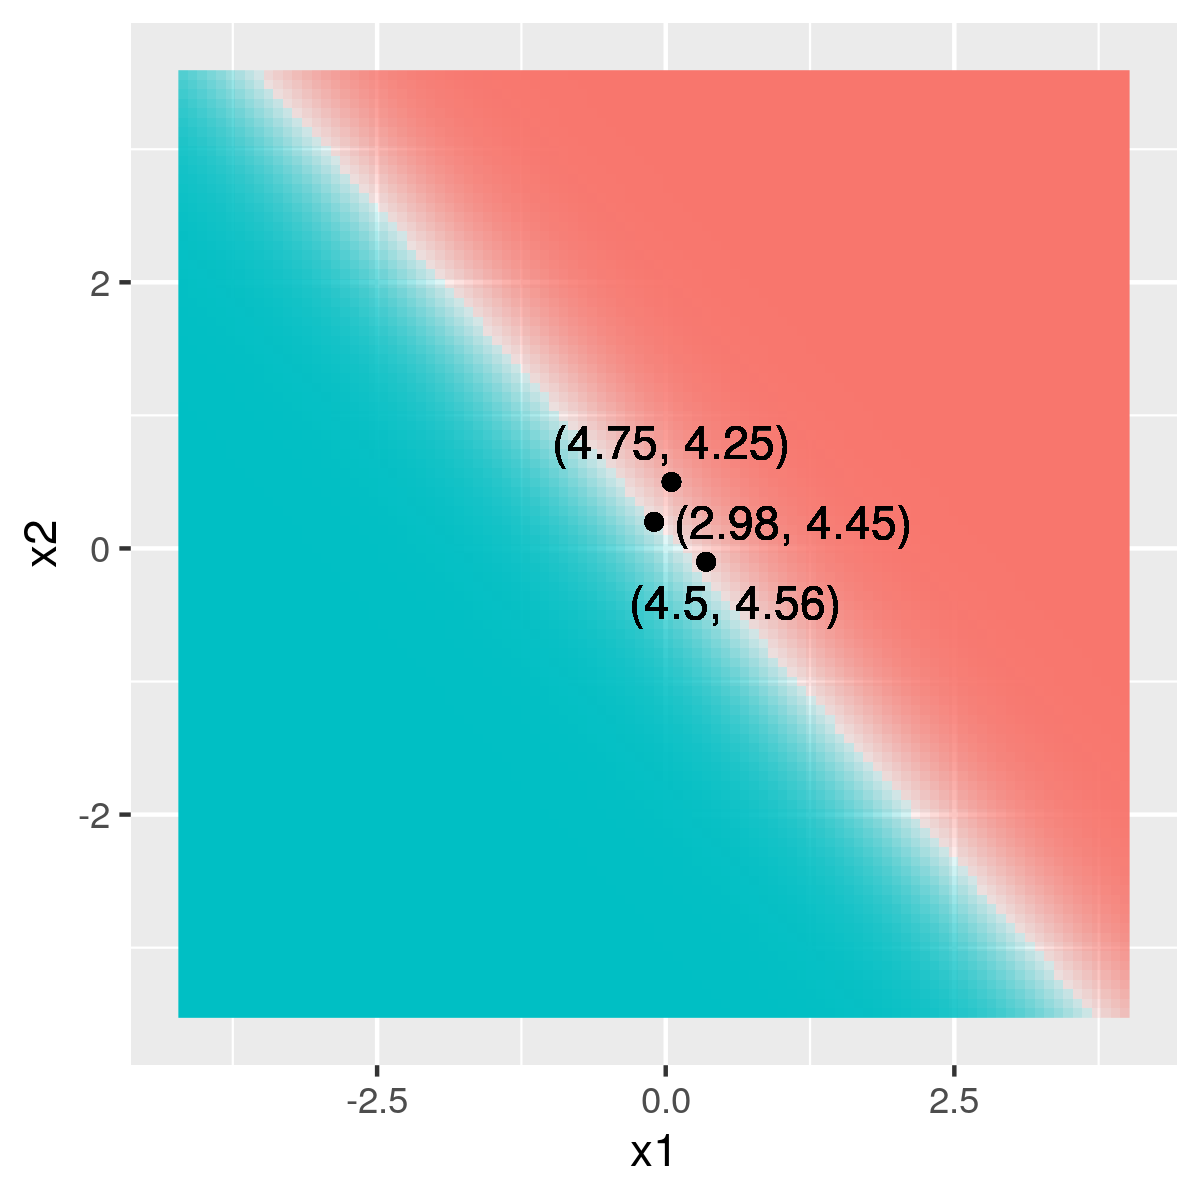
\includegraphics[width=0.5\textwidth]{figure/lime_robustness_1.png}
		
		\tiny{Linear prediction task (logistic regression).\\ Linear surrogate returns similar coefficients for similar points.}
		
		\end{center}
	\end{column}
	\begin{column}{0.48\textwidth}
		\begin{center}
	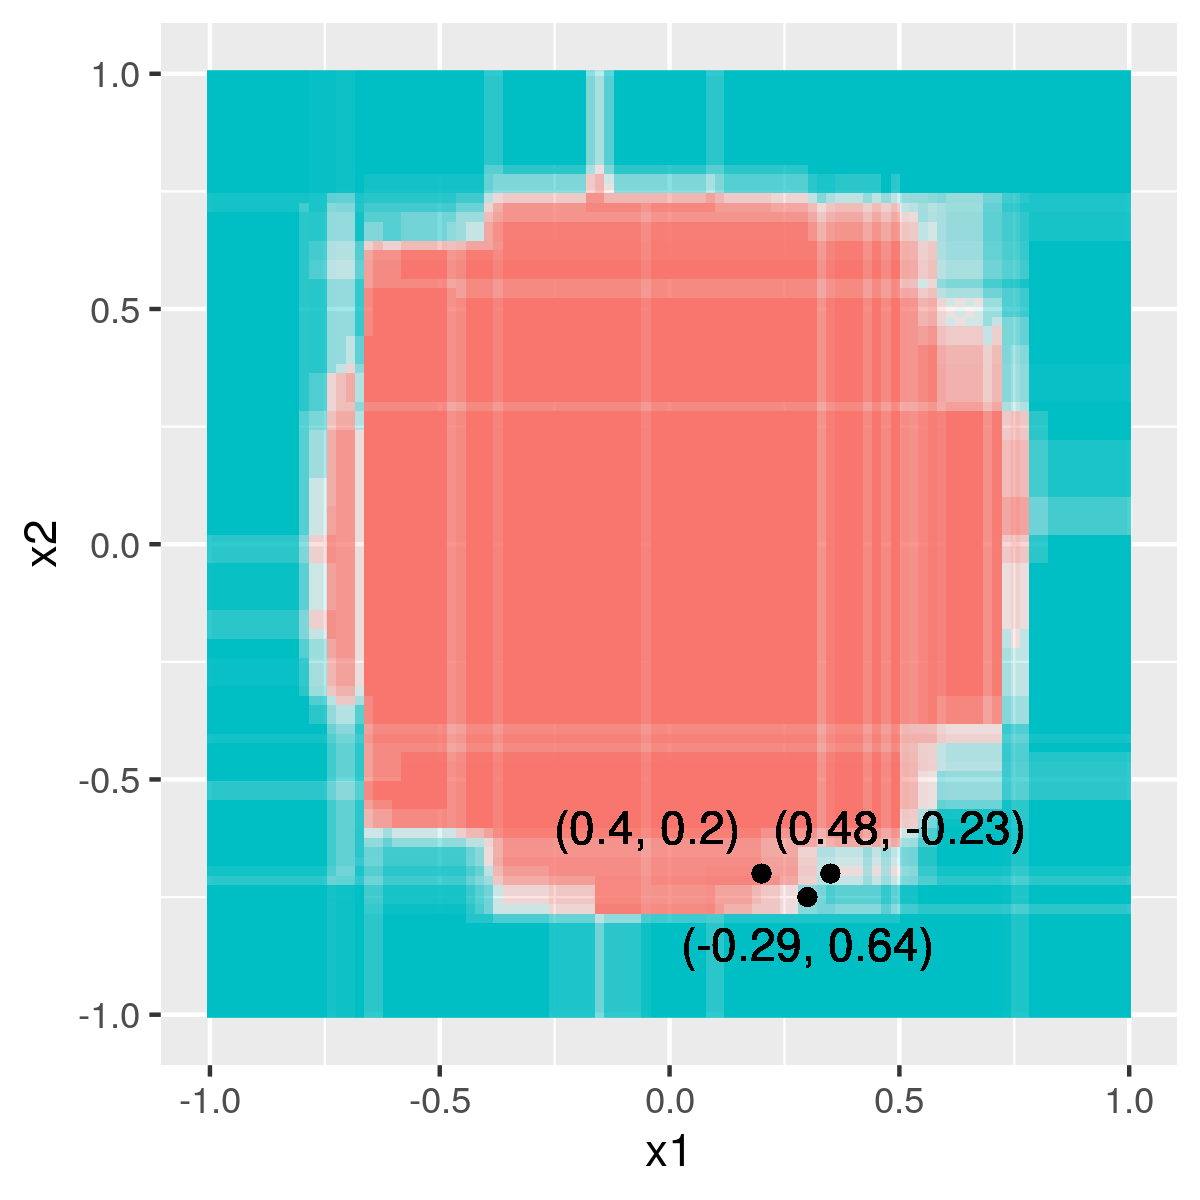
\includegraphics[width=0.5\textwidth]{figure/lime_robustness_2.png}
	
	\tiny{Circular prediction task (random forest).\\ Linear surrogate returns different coefficients for similar points.}
	
	\end{center}
\end{column}
\end{columns}

\end{frame}

\begin{frame}[c]{Conclusion}
% \textbf{Pitfall 7: Definition of superpixels}
% \begin{itemize}
% 	\item Another source of instability concerns the definition of superpixels for image data. 
% 	\item Multiple definitions of superpixels exist and these definitions influence both the shape and size. 
% 	\item The definition of superpixel has a large influence on the explanations. 
% 	\item Furthermore, if superpixel are only slightly changed (adversarial attack), the definitions could still differ greatly.  
% \end{itemize}

%\bigskip
%\pause

{\huge
\alert{LIME (and related approaches) should only be used with great caution.}}

\pause

\bigskip
(This applies to all explainablity techniques ;-) )

\end{frame}


% \begin{frame}{Problems, Pitfalls, \& Limitations of CEs}
% \begin{itemize}
%     \item \textbf{Illusion of model understanding:} 
%     CEs explain ML decisions by pointing to few specific alternatives. This reduces complexity, but is limited in explanatory power. Psychologists showed that even though the perceived model-understanding of end-users increases, the objective model-understanding remains unchanged.
%     \pause
%     \item \textbf{Finding the right metric:} Similarity is the crucial concept for finding good CEs. However, our concept of similarity is context and domain dependent. E.g. while L$_1$ can be a reasonable notion for tabular data, it is counterintuitive for image data. Sparsity is often desirable for end-users but not for data scientists searching for biases in the model.
%     \pause
%     \item \textbf{Confusing Model and Real-World:} As pointed out before, explanations of the model do not easily transfer to the process in which a model is applied. This information should be conveyed to the end-user.
% \end{itemize}
    
% \end{frame}
% \begin{frame}{Problems, Pitfalls, \& Limitations of CEs}
% \begin{itemize}
%     \item \textbf{Disclosing too much information:} CEs can reveal too much information about the model and help potential attackers.
%     \pause
%     \item \textbf{Rashomon effect:} One, few, all? Which CEs should be shown to the end-user? There is no universal solutions, the right way depends on the end-users temporal resources and knowledge. 
%     \pause
%     \item \textbf{Actionability vs. fairness:} Some authors suggest to focus only on the actionability of CEs. However, this counteract functions like contestability. E.g., if ethnicity is not permuted in a CE since it is not actionable this could lead to hiding racial biases in the model.
%     \pause
%     \item \textbf{Attacking CEs:} Researchers can create models with great performance, which generate arbitrary explanations specified by the ML developer. Thus, the question is how faithful CEs are to the models underlying mechanism.
%     \pause
%     \item \textbf{Assumption of constant model:} To provide guidance for the future, CEs assume that their underlying model would not change in the future. However, in reality this assumption is often violated and CEs are not reliable anymore. 
% \end{itemize}

%\end{frame}

\end{document}